\documentclass[11pt]{amsart}
\usepackage[headings]{fullpage}
\usepackage{amssymb,epic,eepic,epsfig,amsbsy,amsmath,amscd,color,graphicx,subcaption,texdraw,bbm,url}
%\usepackage[bb=boondox]{mathalpha} 
%\usepackage[all]{xy}
\usepackage{mathrsfs}
%\usepackage{standalone}
\usepackage[normalem]{ulem}
%\usepackage{comment}
\usepackage{refcheck}
%\usepackage{soul}
\usepackage[final]{pdfpages}
\usepackage{tikz}
\usetikzlibrary{cd,positioning,knots,patterns,hobby,math,decorations,decorations.markings,arrows.meta}

\theoremstyle{plain}
\newtheorem{theorem}{Theorem}[section]
\newtheorem{thm}{Theorem}
\newtheorem{lemma}[theorem]{Lemma}
\newtheorem{corollary}[theorem]{Corollary}
\newtheorem{proposition}[theorem]{Proposition}
\newtheorem{conjecture}{Conjecture}
\newtheorem{question}{Question}
\newtheorem{claim}[theorem]{Claim}
\newtheorem{definition}{Definition}
\newtheorem{state}{Statement}

\theoremstyle{definition}

\newtheorem{remark}[theorem]{Remark}
\newtheorem{example}[theorem]{Example}
\newcommand{\bcon}{\begin{conjecture}}
\newcommand{\econ}{\end{conjecture}}
\newcommand{\bcor}{\begin{corollary}}
\newcommand{\ecor}{\end{corollary}}
\newcommand{\bdf}{\begin{definition}}
\newcommand{\edf}{\end{definition}}
\newcommand{\benu}{\begin{enumerate}}
\newcommand{\eenu}{\end{enumerate}}
\newcommand{\beq}{\begin{equation}}
\newcommand{\eeq}{\end{equation}}
\newcommand{\bexa}{\begin{example}}
\newcommand{\eexa}{\end{example}}
\newcommand{\bexe}{\begin{exercise}}
\newcommand{\eexe}{\end{exercise}}
\newcommand{\bfac}{\begin{fact}}
\newcommand{\efac}{\end{fact}}
\newcommand{\bite}{\begin{itemize}}
\newcommand{\eite}{\end{itemize}}
\newcommand{\blem}{\begin{lemma}}
\newcommand{\elem}{\end{lemma}}
\newcommand{\bmat}{\begin{pmatrix}}
\newcommand{\emat}{\end{pmatrix}}
\newcommand{\bprb}{\begin{problem}}
\newcommand{\eprb}{\end{problem}}
\newcommand{\bpro}{\begin{proposition}}
\newcommand{\epro}{\end{proposition}}
\newcommand{\bprof}[1]{\noindent{\it Proof of #1:}}
\newcommand{\bque}{\begin{question}}
\newcommand{\eque}{\end{question}}
\newcommand{\brem}{\begin{remark}}
\newcommand{\erem}{\end{remark}}
\newcommand{\bthm}{\begin{theorem}}
\newcommand{\ethm}{\end{theorem}}

\newcommand{\bpr}{\begin{proof}}
\newcommand{\epr}{\end{proof}}
\newcommand{\ignore}[1]{}
\newcommand{\xra}{\xrightarrow}
\newcommand{\hra}{\hookrightarrow}
\newcommand{\lb}{\label}
\newcommand{\la}{\langle}
\newcommand{\ra}{\rangle}

%%%%%%%%%%%

\def\nc{\newcommand}

\newcommand\FIGc[3]{\begin{figure}[htpb]
    \includegraphics[height=#3]{draws/#1.eps}
    \caption{#2}
    \label{fig:#1}
    \end{figure}}


\newcommand\incl[2]{{\includegraphics[height=#1]{#2.eps}}}

\newcommand\incljpg[2]{
\raisebox  {- .49 \height}
{\includegraphics[height=#1]{draws/#2.jpg}}
}
\def\bdD{{\mathbf D}}
\def\cD{\mathcal D}

\newcommand{\diag}[2]{\raisebox{-.5\height}{\includegraphics[height=#2]{#1}}}

%%%%%%%%%%%%%%%%%%%%%%%
\def\BA{\mathbb A}
\def\BC{\mathbb C}
\def\BN{\mathbb N}
\def\BZ{\mathbb Z}
\def\BR{\mathbb R}
\def\BT{\mathbb T}
\def\BQ{\mathbb Q}

\def\N{\mathbb N}
\def\Z{\mathbb Z}
\def\C{\mathbb C}
\def\Q{\mathbb Q}

\def\fb{\mathfrak b}
\def\fp{\mathfrak p}
\def\ft{\mathfrak t}
\def\sl{{\mathfrak{sl}}}

\def\ov{\overline}

\def\al{\alpha}
\def\ve{\varepsilon}
\def\cS{\mathscr S}
\def\bcS{\overline{\mathscr{S}} }

\def\embed{\hookrightarrow}
\def\SL{\mathrm{SL}}

\def\p{\partial}
\def\ab{\mathrm{ab}}
\def\SM{(\Sigma,\cP)}
\def\pS{\partial \Sigma}
\def\btau{\bar \tau}
\def\ooS{\mathring {\cS}}
\def\id{\mathrm{id}}
\def\Dess{\D_{\mathrm{ess}}}
\def\np{\newpage}
\def\pM{\partial M}
\def\cI{\mathcal I}
\def\cN{\mathcal N}
\def\MN{(M,\cN)}
\def\tiX{\widetilde {\sX}}
\def\tcS{\widetilde \cS}
\def\tF{\tilde F}
\def\tPhi{\widetilde{\Phi}}
\def\XD{\sX(\D)}
\def\vpD{\vp_\D}
\def\vpDp{\vp_{\D'}}
\def\Hu{{\cH}}
\def\Hm{\cH_\bullet}
\def\ZD{\CZ(\D)}
\def\LMN{\cT\MN}
\def\fr{\operatorname{fr}}
\def\Splus{\cS^+}
\def\cB{\mathcal B}
\def\Cx{{\BC^\times}}
\def\ord{\mathrm{ord}}
\def\Sx{\cS_\xi}
\def\cL{\mathcal L}
\def\cT{\mathcal T}
\def\hPhi{\hat \Phi}
\def\Col{\text{Col}}

\def\Se{\cS_\ve}
\def\Sx{\cS_\xi}
\def\tSe{\widetilde{\cS}_\ve}
\def\tSx{\widetilde{\cS}_\xi}
\def\Rel{\mathrm{Rel}}
\def\MNp{(M',\cN')}
\def\ocP{\mathring {\cP}}
\def\PDDp{\Psi_{\D,\D'}}
\def\PSSp{\PSi_{\Sigma,\Sigma'}}
\def\cSp{\cS^+}
\def\cD{\mathcal D}
\def\chL{\check L}

\def\be{\begin{equation}}

\def\ee{\end{equation}}

\usepackage{hyperref}
\hypersetup{
    colorlinks=true,
    linkcolor=blue,
    filecolor=magenta,      
    urlcolor=cyan,
    pdftitle={Overleaf Example},
    pdfpagemode=FullScreen,
    }

\urlstyle{same}


\def\Mod{{\mathsf {Mod}}}
\def\LMod{{\mathsf {LMod}}}
\def\RMod{{\mathsf {RMod}}}
\def\LMC{\LMod_\CC}
\def\RMC{\RMod_{\CC}}
\def\End{{\mathsf{End}}}
\def\ot{{\otimes}}
\def\CM{{\mathcal M}}
\def\CA{{\mathcal A}}
\def\CE{{\mathcal E}}
\def\CN{{\mathcal N}}
\def\op{\mathrm{op}}
\def\uF{{\underline F}}

\def\fg{{\mathfrak{g}}}
\def\UAg{{U_\CA(\fg)}}
\def\UA{{U_\CA}}

\def\UR{{U_R}}
\def\Ck{{\CC_k}}

\def\Uxi{{U_\xi}}
\def\Cxi{{\CC_\xi}}
\def\tCxi{{\tilde\CC_\xi}}
\def\Obj{{\mathsf {Obj}}}
\def\tR{{\tilde R}}
\def\comod{\text{-comod}}
\def\CCf{{\CC}^f}
\def\hC{\hat{\CC}^f}
\def\Rib{{{\mathcal R}ib}}
\def\Ccomod{{\cH\text{-coMod}}}

\def\coinv{{\mathsf{coinv}}}
\def\CH{{\mathcal H}}


\def\inv{{\mathsf{inv}}}
\def\Cut{{\mathsf{Cut}}}

\def\hxi{{\hat \xi}}
\def\cA{{\mathcal A}}

\def\Zq{{\BZ[q^{\pm 1}]}}
\def\Zhq{{\BZ[\hq^{\pm 1}  ]}}
\def\Zv{{\BZ[v^{\pm 1}]}}

\def\hq{{\hat q}}
\def\Zv{{\BZ[v^{\pm 1}]}}
\def\Qv{{\BQ(v)}}

\def\AU{{_\cA \Ud}}
\def\AMs{{_\cA M_*}}
\def\AM{{_\cA M}}
\def\Qq{\BQ(\hq)}

\def\Rep{{\mathsf{Rep}}}
\def\Oq{{\mathcal O_q}}

\def\bbeta{\boldsymbol{\beta}}  
\def\scrB{\mathscr{B}} 
\def\scrC{\mathscr{C}} 
\def\bSS{\overline{\cS}(\fS)}
\def\bSSQ{\overline{\cS}(\fS)_\BQ}  

\def\g{{\mathfrak g}}

\def\U{{ {\mathcal U}}}
\def\Uc{{\check {\mathcal U}}}
\def\Ucg{\Uc_q(gl_n)}

\def\UcB{ \Uc^{\ge   }}
\def\UcBn{ \Uc^{\le}}
\newcommand{\lf}{{l\! f}}
\def\Ulf{\U^{l\! f}}
\def\Uclf{\Uc^{l\! f}}

\def\O{{\mathcal O}}
\def\TO{\mathcal T\O}


\def\Ud{{\dot{\mathcal U}}}
\def\Urat{{\Ud^{ \mathsf {rat  }  }}}
\def\Uhxi{{\dot{\mathcal U}}_\hxi}
\def\UcA{_\cA\Uc}


\def\bS{\overline \CS}

\def\SS{{\cS(\fS)}}
\def\fB{\mathfrak B}

\def\onto{\twoheadrightarrow}

\def\binv{{\overline{\mathsf{inv}  }_{ e_l }}}

\def\glue{{\mathsf{glue}}}

\def\buu{{\mathbf  u}}

\def\bipr{{
  \triangleright\mathrel{\mkern-12mu}
  \triangleleft}}
  
 \def\INV{{\mathsf{INV}}}
\def\tm{{\mathsf{tm}}}
\def\pmo{{\pm 1}}
\def\mpo{{\mp 1}}
\def\K{\mathbb K}

\newcommand{\red}[1]{{\color{red}#1}}

%%%%%%%%%%%%%%%%%%%%%%%%%%%%%%%%%%%%%%%%%%%%%

\tikzset{edge/.style={line width=0.8}}
\tikzset{wall/.style={very thick}} 
\tikzset{->-/.style n args={2}{decoration={markings, mark=at position #1 with {\arrow{#2}}}, postaction={decorate}}}

\ExplSyntaxOn
\cs_new_eq:NN \ifstreqF \str_if_eq:nnF
\cs_new_eq:NN \ifstreqTF \str_if_eq:nnTF
\ExplSyntaxOff

\tikzset{-o-/.code 2 args={\ifstreqF{#2}{}
{\ifstreqTF{#2}{>}
   {\pgfkeysalso{decoration={markings,mark=at position #1 with {\arrow[scale=0.8]{#2}}}
                    ,postaction={decorate}}
    }
   {\ifstreqTF{#2}{<}
       {\pgfkeysalso{decoration={markings,mark=at position #1 with {\arrow[scale=0.8]{#2}}}
                    ,postaction={decorate}}
        }
       {\pgfkeysalso{decoration={markings,
                    mark=at position #1 with 
                    {\draw[black, fill={#2}] circle[radius=2pt];}}
                    ,postaction={decorate}}
        }
     }
  }}} 


\newcommand{\bigonpicold}[6]{ 
\raisebox{-0.4\height}{\begin{tikzpicture}
        \tikzmath{\xdim=#4; \ydim=#5; \h=0.5; \o=\ydim/2; \t1=\ydim/3; \t2=\ydim*2/3;} 
        \ifthenelse{\equal{#3}{b}}{
         \fill[gray!20!white, rounded corners=1.5mm]  (\xdim/2, -\h)-- (0,0)--(0,\ydim) -- (\xdim/2, \ydim+\h) -- 
         (\xdim,\ydim)  -- (\xdim,0) -- cycle;
          \draw[wall,  -o-={.3}{#1}, rounded corners=1.5mm] (\xdim/2, -\h)-- (0,0)--(0,\ydim) -- (\xdim/2, \ydim+\h);
       \draw[wall, -o-={.3}{#2}, rounded corners=1.5mm] (\xdim/2, -\h)-- (\xdim,0)--(\xdim,\ydim) -- (\xdim/2, \ydim+\h);
        \draw[black, fill=white] (\xdim/2,\ydim+\h) circle[radius=2pt];
        }
        {\draw[wall,  -o-={.51}{#1}, fill=gray!20!white]  
        (\xdim/2, -\h) [rounded corners=1.5mm] --  (0,0) [sharp corners] --(0,\ydim) 
        arc [start angle =180, end angle =0, radius=\xdim/2] 
         [rounded corners=1.5mm]  --(\xdim,0) [sharp corners] -- cycle;} 
        \draw[black, fill=white] (0.5*\xdim,-\h) circle[radius=2pt];
          #6
\end{tikzpicture}
}\hspace*{-.1in}} 


\newcommand{\bigonalpha}[6]{ 
\bigonpicold{#1}{#2}{#3}{0.8}{.6}{
\coordinate[label={left:{\small #5}}] (A) at (0,\o); 
\coordinate[label={right:{\small #6}}] (B) at (\xdim,\o);
\node [thick, circle, draw, fill=white, radius=0.5] (N) at (\xdim/2,\o) {\hspace*{-.1in}#4\hspace*{-.1in}};
\draw[edge] (0,\o) -- (N);
\draw[edge] (N) -- (\xdim,\o);
}
}

\newcommand{\BigonP}[3]{
\begin{tikzpicture}[baseline=.6ex, scale=#1]
    \fill[gray!20] (0,2) to[bend left=90] (0,-2) to[bend left=90] (0,2);
    \draw[thick, #2] (0,2) to[bend left=90] (0,-2);
    \draw[thick, #2] (0,2) to[bend right=90] (0,-2);
    \fill[draw=black, fill=white] (0,2) circle (0.2);
    \fill[draw=black, fill=white] (0,0) circle (0.2);
    \fill[draw=black, fill=white] (0,-2) circle (0.2);
    #3
\end{tikzpicture}
}

\def\BigonPlines{
\BigonP{0.35}{}{
\draw[draw=blue, thick]  (-1.1, 0.8) -- (1.1, 0.8);
\draw[draw=blue, thick]  (-1.1, -0.8) -- (1.1, -0.8);
}
}

\def\BigonPGens{ 
\BigonP{.50}{decoration={markings, mark=at position 0.8 with {\arrow{>}}}, postaction={decorate}}{
\draw[draw=blue, thick, decoration={markings, mark=at position 0.5 with {\arrow{>}}}, postaction={decorate}]  (-1.1, 0.55) -- (1.1, 0.55);
\draw[draw=blue, thick, decoration={markings, mark=at position 0.5 with {\arrow{>}}}, postaction={decorate}]  (-1.1, -0.55) -- (1.1, -0.55);
\node[anchor=east] at (-1.1, 0.55) {$k$};
\node[anchor=west] at (1.1, 0.55) {$l$};
\node[anchor=east] at (-1.1, -0.55) {$i$};
\node[anchor=west] at (1.1, -0.55) {$j$};
\node[anchor=south] at (0, 0.55) {$c_{kl}$};
\node[anchor=north] at (0, -0.55) {$b_{ij}$};
}
}

 \def\punctbigonweb{
 \BigonP{.5}{decoration={markings, mark=at position 0.9 with {\arrow{>}}}, postaction={decorate}}{
 \draw[draw=blue] ellipse (0.7 and 1.5);
 \node[anchor=south] at (0, 0.1) {\color{blue} $\beta$};
  \draw[draw=blue, thick] (-1.1, 0.8) -- (-0.65, 0.7);
    \draw[draw=blue, thick] (-1.1,-0.8) -- (-0.65,-0.7);
    \node[left]  at (-1.1, 0.8) {$i_k$};
    \node[left]  at (-1.1, -0.8) {$i_1$};
    
    \foreach \y in {-0.25,0,0.25}
        \fill[blue] (-1,\y) circle (1.5pt);

    \draw[draw=blue, thick] (0.65, 0.7) -- (1.1, 0.8);
    \draw[draw=blue, thick] (0.65,-0.7) -- (1.1,-0.8);
    \node[right]  at (1.1, 0.8) {$j_l$};
    \node[right]  at (1.1, -0.8) {$j_1$};

    \foreach \y in {-0.25,0,0.25}
        \fill[blue]  (1,\y) circle (1.5pt);
 }
 }
 
 \def\punctbigonwebS{
 \BigonP{.5}{decoration={markings, mark=at position 0.9 with {\arrow{>}}}, postaction={decorate}}{
 \draw[draw=blue] ellipse (0.7 and 1.5);
 \node[anchor=north] at (0, 0.1) {\color{blue} \rotatebox[origin=c]{180}{$\beta$}};
  \draw[draw=blue, thick] (-1.1, 0.8) -- (-0.65, 0.7);
    \draw[draw=blue, thick] (-1.1,-0.8) -- (-0.65,-0.7);
    \node[left]  at (-1.1, 0.8) {$\overline{j_1}$};
    \node[left]  at (-1.1, -0.8) {$\overline{j_l}$};

    \foreach \y in {-0.25,0,0.25}
        \fill[blue] (-1,\y) circle (1.5pt);

    \draw[draw=blue, thick] (0.65, 0.7) -- (1.1, 0.8);
    \draw[draw=blue, thick] (0.65,-0.7) -- (1.1,-0.8);
    \node[right]  at (1.1, 0.8) {$\overline{i_1}$};
    \node[right]  at (1.1, -0.8) {$\overline{i_k}$};

    \foreach \y in {-0.25,0,0.25}
        \fill[blue]  (1,\y) circle (1.5pt);
 }
 }

\def\BigonPpm{ 
\BigonP{.6}{decoration={markings, mark=at position 0.8 with {\arrow{>}}}, postaction={decorate}}{
\draw[draw=blue, thick, decoration={markings, mark=at position 0.5 with {\arrow{>}}}, postaction={decorate}]  (-1.1, 0.55) -- (1.1, 0.55);
\draw[draw=blue, thick, decoration={markings, mark=at position 0.5 with {\arrow{>}}}, postaction={decorate}]  (-1.1, -0.55) -- (1.1, -0.55);
\node[anchor=south] at (0, 0.55) {$\fB^-$};
\node[anchor=north] at (0, -0.55) {$\fB^+$};
}
}

\newcommand{\BigonXY}[1]{
\begin{tikzpicture}[ baseline=.6ex, scale=#1, line cap=round, line join=round]

    \fill[gray!20] (0,2) .. controls (1.85,1.55) and (1.85,-1.55) .. (0,-2)
        .. controls (-1.85,-1.55) and (-1.85,1.55) .. cycle;
        
    \draw[ blue, line width=1.2pt, name path=understrand]
        (-1.40,.31) .. controls (-.01,-1.31) and (-.35,-1.75) .. (1.04,-.25) -- (1.40,.28);
 
    \path[name path=overstrand]
        (-1.39,-.42)  .. controls (-.09,1.06) and (.19,1.10) .. (1.40,-.42);
 
    \path[name intersections={of=understrand and overstrand, name=crossing} ];
    \foreach \k in {1,2}
        \fill[gray!20] (crossing-\k) circle[radius=.15];

    \draw[blue,line width=1.2pt] (-1.39,-.42) .. controls (-.09,1.06) and (.19,1.10) .. (1.40,-.42);
    
    \draw[thick, decoration={markings, mark=at position 0.8 with {\arrow{>}}}, postaction={decorate}] 
        (0,2)  .. controls (1.85,1.55) and (1.85,-1.55) .. (0,-2);
    \draw[thick, decoration={markings, mark=at position 0.8 with {\arrow{>}}}, postaction={decorate}] 
        (0,2) .. controls (-1.85,1.55) and (-1.85,-1.55) .. (0,-2);
      
    \filldraw[ fill=white, draw=blue, line width=1.2pt ] (0,.69) ellipse[x radius=.53,y radius=.39];

    \node at (0,.69) {$x^{-}$};

    \filldraw[fill=white,draw=blue, line width=1.2pt] (0,-.90) ellipse[x radius=.53,y radius=.39];

    \node at (0,-.90) {$x^{+}$};

    \foreach \p in {(0,2),(0,0),(0,-2)}
        \filldraw[ fill=white, draw=black, line width=.6pt] \p circle[radius=.13];
\end{tikzpicture}
}

\newcommand{\Bigonbc}[5]{
\begin{tikzpicture}[baseline=.6ex, scale=#1, line cap=round, line join=round]
 
    \fill[gray!20] (0,2) .. controls (1.85,1.55) and (1.85,-1.55) .. (0,-2) .. controls (-1.85,-1.55) and (-1.85,1.55) .. cycle;
    
    \draw[blue, line width=.8pt, decoration={markings, mark=at position .5 with {\arrow{>}}}, postaction={decorate}] (-1.4,.6) -- (1.4,.6);
     \node[anchor=east] at (-1.4, 0.6) {#2};
     \node[anchor=west] at (1.4, 0.6) {#3};
 
    \draw[blue, line width=.8pt, decoration={markings, mark=at position .5 with {\arrow{>}}}, postaction={decorate}] (-1.4,-.6) -- (1.4,-.6);
    \node[anchor=east] at (-1.4, -0.6) {#4};
     \node[anchor=west] at (1.4, -0.6) {#5};
     
    \draw[thick, decoration={markings, mark=at position 0.8 with {\arrow{>}}}, postaction={decorate}]
        (0,2) .. controls (1.85,1.55) and (1.85,-1.55) .. (0,-2);

    \draw[thick, decoration={markings, mark=at position 0.8 with {\arrow{>}} }, postaction={decorate}]
        (0,2) .. controls (-1.85,1.55) and (-1.85,-1.55) .. (0,-2);

    \foreach \p in {(0,2),(0,0),(0,-2)}
        \filldraw[ fill=white, draw=black, line width=.6pt] \p circle[radius=.13];
\end{tikzpicture}
}


\newcommand{\BigonbcXX}[1]{
\begin{tikzpicture}[baseline=.6ex, scale=#1, line cap=round, line join=round]
 
    \fill[gray!20] (0,2) .. controls (1.85,1.55) and (1.85,-1.55) .. (0,-2) .. controls (-1.85,-1.55) and (-1.85,1.55) .. cycle;
    
    \draw[blue, line width=1pt, name path=understrand, decoration={markings, mark=at position 0.8 with {\arrow{>}}}, postaction={decorate}]
        (-1.40,.31) .. controls (-.01,-1.31)  .. (1.04,-.25) .. controls (1.16,-.12) and (1.2,.10) .. (1.40,.28);
     \node[anchor=east] at (-1.4, 0.4) {$i$};
     \node[anchor=west] at (1.4, 0.4) {$j$};
 
    \path[name path=overstrand] (-1.39,-.42)  .. controls (-.09,1.06) and (.19,1.10) .. (1.40,-.42);
    \node[anchor=east] at (-1.4, -0.4) {$k$};
     \node[anchor=west] at (1.4, -0.4) {$l$};

    \path[name intersections={of=understrand and overstrand,name=crossing}];

    \foreach \k in {1,2}
     \fill[gray!20] (crossing-\k) circle[radius=.15];

    \draw[blue,line width=1pt, decoration={markings, mark=at position 0.8 with {\arrow{>}}}, postaction={decorate}]
        (-1.39,-.42)
        .. controls (-.09,1.06) and (.19,1.10) .. (1.40,-.42);

    \draw[thick, decoration={markings, mark=at position 0.8 with {\arrow{>}}}, postaction={decorate}]
        (0,2) .. controls (1.85,1.55) and (1.85,-1.55) .. (0,-2);

    \draw[ thick, decoration={markings, mark=at position 0.8 with {\arrow{>}} }, postaction={decorate}]
        (0,2) .. controls (-1.85,1.55) and (-1.85,-1.55) .. (0,-2);

    \foreach \p in {(0,2),(0,0),(0,-2)}
        \filldraw[ fill=white, draw=black, line width=.6pt] \p circle[radius=.13];
\end{tikzpicture}
}

\def\Ci{
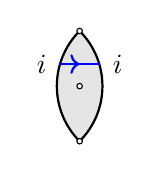
\begin{tikzpicture}[baseline=.6ex, scale=0.35]

    \fill[gray!20] (0,2) to[bend left=45] (0,-2) to[bend left=45] (0,2);
    \draw[thick] (0,2) to[bend left=45] (0,-2);
    \draw[thick] (0,2) to[bend right=45] (0,-2);
    
    \draw[thick, draw=blue, decoration={markings, mark=at position 0.5 with {\arrow{>}}}, postaction={decorate}] 
        (-0.75, 0.8) -- (0.75, 0.8);

    \fill[draw=black, fill=white] (0,2) circle (0.1);
    \fill[draw=black, fill=white] (0,0) circle (0.1);
    \fill[draw=black, fill=white] (0,-2) circle (0.1);
    
     \node[anchor=east] at (-0.85, 0.8) {$i$};
    \node[anchor=west] at (0.85, 0.8) {$i$};
\end{tikzpicture}
}

\def\Bin{
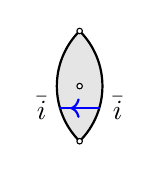
\begin{tikzpicture}[baseline=.6ex, scale=0.35]
    {}
    \fill[gray!20] (0,2) to[bend left=45] (0,-2) to[bend left=45] (0,2);
    \draw[thick] (0,2) to[bend left=45] (0,-2);
    \draw[thick] (0,2) to[bend right=45] (0,-2);

    {}
    \draw[thick, draw=blue, decoration={markings, mark=at position 0.5 with {\arrow{<}}}, postaction={decorate}] 
        (-0.75, -0.8) -- (0.75, -0.8);

    {}
    \fill[draw=black, fill=white] (0,2) circle (0.1);
    \fill[draw=black, fill=white] (0,0) circle (0.1);
    \fill[draw=black, fill=white] (0,-2) circle (0.1);

    {}
     \node[anchor=east] at (-0.85, -0.8) {$\bar i$};
    \node[anchor=west] at (0.85, -0.8) {$\bar i$};
\end{tikzpicture}
}

\newcommand{\Ei}[4]{
\begin{tikzpicture}[baseline=.6ex, scale=0.45]
    \fill[gray!20] (0,2) to[bend left=45] (0,-2) to[bend left=45] (0,2);
    \draw[thick, decoration={markings, mark=at position 0.9 with {\arrow{>}}}, postaction={decorate}] (0,2) to[bend left=45] (0,-2);
    \draw[thick, decoration={markings, mark=at position 0.9 with {\arrow{>}}}, postaction={decorate}] (0,2) to[bend right=45] (0,-2);

    \draw[thick, draw=blue, decoration={markings, mark=at position 0.5 with {\arrow{>}}}, postaction={decorate}] 
        (-0.75, 0.9) -- (0.75, 0.9);
    \draw[thick, draw=blue, decoration={markings, mark=at position 0.5 with {\arrow{<}}}, postaction={decorate}] 
        (-0.85, 0.2) -- (0.85, 0.2);
        
    \fill[draw=black, fill=white] (0,2) circle (0.1);
    \fill[draw=black, fill=white] (0,-0.3) circle (0.1);
    \fill[draw=black, fill=white] (0,-2) circle (0.1);

    \node[anchor=east] at (-0.85, 1) {#1};
    \node[anchor=west] at (0.85, 1) {#2};
    \node[anchor=east] at (-0.85, 0) {#3};
    \node[anchor=west] at (0.85, 0) {#4};
\end{tikzpicture}
}

\newcommand{\Fi}[4]{
\begin{tikzpicture}[baseline=.6ex, scale=0.45]
  
    \fill[gray!20] (0,2) to[bend left=45] (0,-2) to[bend left=45] (0,2);
    \draw[thick,decoration={markings, mark=at position 0.9 with {\arrow{>}}}, postaction={decorate}] (0,2) to[bend left=45] (0,-2);
    \draw[thick, decoration={markings, mark=at position 0.9 with {\arrow{>}}}, postaction={decorate}] (0,2) to[bend right=45] (0,-2);

    \draw[thick, draw=blue, decoration={markings, mark=at position 0.5 with {\arrow{>}}}, postaction={decorate}] 
        (-0.75, -0.8) -- (0.75, -0.8);
    \draw[thick, draw=blue, decoration={markings, mark=at position 0.5 with {\arrow{<}}}, postaction={decorate}] 
        (-0.85, -0.2) -- (0.85, -0.2);

    \fill[draw=black, fill=white] (0,2) circle (0.1);
    \fill[draw=black, fill=white] (0,.3) circle (0.1);
    \fill[draw=black, fill=white] (0,-2) circle (0.1);
    
    \node[anchor=east] at (-0.85, 0) {#1};
    \node[anchor=west] at (0.85, 0) {#2};
    \node[anchor=east] at (-0.85, -1) {#3};
    \node[anchor=west] at (0.85, -1) {#4};
\end{tikzpicture}
}

\newcommand{\upperbigoncross}[1]{
\begin{tikzpicture}[scale=#1]
   
    \fill[gray!30]
        (0,2)
        .. controls (-1.25,1.35) and (-1.45,0.55) .. (-1.35,0)
        .. controls (1.35,0) .. (1.35,0)
        .. controls (1.45,0.55) and (1.25,1.35) .. cycle;        
    \draw[thick, draw=blue] (-0.90,1.35) -- (1.35,0.10);

\draw[gray!30, line width=5pt]  (-1.35,0.25) -- (1,1.3);

\draw[thick, draw=blue] (-1.35,0.25) -- (0.95,1.3);    

    \draw[thick] (0,2) .. controls (-1.25,1.35) and (-1.45,0.55) .. (-1.35,0);
    \draw[thick] (0,2) .. controls (1.25,1.35) and (1.45,0.55) .. (1.35,0);

    \filldraw[fill=white, thick] (0,2) circle (0.13);
  
    \node[left]  at (-1.35,0) {$k$};
    \node[right] at (1.35,0) {$j$};
    \node[left]  at (-0.85,1.55) {$i$};
    \node[right] at (0.95,1.55) {$\ell$};
\end{tikzpicture}
}

\newcommand{\Rform}[2]{
\begin{tikzpicture}[ scale=.4, baseline=(current bounding box.center),
    line width=1.5pt,
    >={Stealth[length=3mm,width=2mm]},
    bg/.style={black!12},
    bubble/.style={circle, draw, line width=1.5pt,
                   inner sep=0pt, minimum size=0.6cm, fill=black!12}
  ]

  \fill[bg] (0,0.4) rectangle (4.3,-4.3);

  \node[bubble] (x) at (1.25,-1.2) {#1};
  \node[bubble] (y) at (1.25,-3) {#2};

  \draw (0,-1.2) -- (x.west);
  \draw (0,-3) -- (y.west);

  \draw (y.east) .. controls (2.6,-3) and (2.9,-1.8) .. (4.4,-0.95);

  \draw[preaction={draw,line width=8pt,bg}]
        (x.east) .. controls (2.6,-1.2) and (2.9,-2.9) .. (4.4,-3.75);
        
  \draw[->] (0,0.4) -- (0,-5);
  \draw[->] (4.4,0.4) -- (4.4,-5);        

\end{tikzpicture}
}


\newcommand{\gray}[1]{{\color{blue}#1}}

%%%%%%%%%%%%%%%%%%%%%%%%%%%%%%%%%%%%%%%%%%%%%%%%%%%%%%%
\begin{document}
\begin{center}
{\large Adam Sikora}
\end{center}
\section{Algebraic Preliminaries}

%%%%%%%%%%%%%%%%%%%%%%%%%%%%%%%%%%%%%%%%%%%%%
\subsection{Double cross product, quantum double} In this subsection, we follow \cite{Majid2}, \cite[Section 8.2]{KS}. 

 A {\em skew pairing} of two bialgebras $A,B$ over a field $\K$, is a bilinear form $\sigma: A \ot_\K B \to \K$ satisfying
\begin{align}
\sigma(a\ot 1) & = \epsilon_A(a),\quad  \sigma( 1 \ot b)  = \epsilon_B(b )\label{e.pairing1}\\
\sigma(a\cdot a', b )&= \sum \sigma(a, b_{(1)})\cdot \sigma (a', b_{(2)}) \\
\sigma(a, b\cdot b')&= \sum \sigma ( a_{(2)},b)\cdot \sigma (a_{(1)},b').\label{e.pairing3} 
\end{align}
(Note that a skew pairing differs from a Hopf pairing by switching $a_{(1)}$ and $a_{(2)}$ in the last identity.) 

Assume now that $A,B$ are Hopf algebras with invertible antipodes. Then any pairing $\sigma$ between them has an inverse
$$\bar \sigma(a\ot b) = \sigma(S(a), b) = \sigma(a, S^{-1}(b))$$
and the {\em double cross product} $B \, \bipr _\sigma A$, is the algebra $B \ot A$, with the product such that the linear embeddings $A \embed B \ot A, a \to 1\ot a$ and $B \embed B \ot A, b \to b\ot 1$ are algebra maps and
\begin{align}
b a &= b \ot a \label{e.ba}\\
ab &= \sum \bar \sigma(a_{(1)} \ot b_{(1)}) \sigma(a_{(3)} \ot b_{(3)}) \, b_{(2)} a_{(2)},\label{e.ab}
\end{align}
for $a\in A \subset B \ot A$ and $b \in B \subset B\ot A$.

Furthermore,  $B \, \bipr _\sigma A$ is a Hopf algebra with the coproduct 
$$\nabla(b\ot a)=\sum b_{(1)}\ot a_{(1)}\ot b_{(2)}\ot a_{(2)},$$
and the antipode
$$S(b \ot a)= S(a)S(b).$$


%%%%%%%%%%%%%%%%%%%%%%%%%%%%%%%%%%%%%%%%%%%%%%%%%%%%%%%%%%%%%
\subsection{$U_q(\sl(n))$ and its simply-connected and De Concini-Procesi versions}
\label{ss.Uq}

Let $\Uc=\check U_q(\sl(n))$ be the simply-connected quantized enveloping algebra of $\sl(n)$, over $\K=\Q(v),$ for $n\geq 2$
where $q=v^{2n}$, following \cite{LS}. (For the purpose of this section, one can work over $\Q(v^2)$ instead.)
This algebra is denoted by $U_q^P(\sl(n))$ in \cite{Gavarini2}. 
(The index $n$ is fixed throughout this note and we suppress it for simplicity.)
It is generated by $G_i^{\pm1}, i=1, \dots, n,$ and $E_i, F_i$, $i=1, \dots n-1$ with relations,
$$G_i^{\pm 1}G_j^{\pm 1}=G_j^{\pm 1}G_i^{\pm 1},\qquad G_1 G_2 \dots G_n=1,$$
\beq\label{e.GEF}
G_iE_jG_i^{-1}=q^{\delta_{i,j}-\delta_{i,j+1}}E_j,\quad  G_iF_jG_i^{-1}=q^{\delta_{i,j+1}-\delta_{i,j}}F_j,
\eeq
\beq\label{e.EF}
E_iF_j-F_jE_i=\delta_{i,j}\frac{G_iG_{i+1}^{-1}-  G_i^{-1}G_{i+1}}{q-q^{-1}},
\eeq
$$E_iE_j=E_jE_i,\quad F_i F_j=F_jF_i,\quad \text{for}\ |i-j|>1$$
$$E_i^2E_j-[2] E_iE_jE_i+E_jE_i^2=0=F_i^2F_j-[2] F_iF_jF_i+F_jF_i^2,\quad \text{for}\ |i-j|=1.$$
for all $i,j,$ \cite{Gavarini2}. 
Here we use the standard notation for quantum integers:
$$[m] := \frac{q^m-q^{-m}}{q-q^{-1}}\in \Z[q^\pmo].$$
The generators $G_1,...,G_n$ correspond to the weight of the $n$-dimensional defining representation of $\sl(n)$ and are denoted by $\hat K_1,...,\hat K_n$ in \cite{KS}.
The standard Drinfeld-Jimbo quantum groups $\U=U_q(\sl(n))$ are subalgebras of $\Uc$
generated by $K_i = G_i G_{i+1}^{-1},$ for $i=1,...,n-1$, associated with the simple roots, together with $E_i$'s and $F_i$'s. 

In particular, we have
\beq\label{e.KEF}
K_jE_i=q^{a_{ij}}E_iK_j,
\eeq
for all $i,j,$ where $(a_{ij})$ is the $A_{n-1}$ Cartan matrix, $a_{ii}=2,$ $a_{i,i\pm 1}=-1$ and $a_{i,j}=0$ for  $|i-j|>1.$ 

Following \cite{Kass, KS}, the coproduct and the antipode in $U_q(\sl(n))$ satisfy 

\beq\label{e.copr}
\Delta(K_i)=K_i\ot K_i,\quad \Delta(E_i)=E_i\ot K_i+1\ot E_i,\quad \Delta(F_i)=F_i\ot 1+K_i^{-1}\ot F_i.
\eeq
\beq\label{e.antip}
S(K_i)=K_i^{-1},\quad S(E_i)=-E_i K_i^{-1},\quad S(F_i)=-K_i F_i.
\eeq

\brem\label{r.Gav} Gavarini's quantum groups have the opposite coproduct to those of \cite{Kass,KS} and those used in the theory of skein algebras, eg. \cite{LS}.
Consequently, Gavarini's formulas in this paper are transformed through the Cartan involution, which is an algebra homomorphism and coalgebra anti-homomorphism.  
\beq\label{e.Cartan}
\phi(E_i) = F_i,\quad \phi(F_i) = E_i,\quad \phi(G_i) = G_i^{-1}.
\eeq
\erem

\def\Op{{\O^{\ge}}}
\def\On{{\O^{\le}}}

The positive Borel subalgebra $\Uc^{\ge }\subset \Uc$ is the $\Qv$-subalgebra generated by $G_i^{\pm 1},$ for $i=1, \dots , n$ and by $E_i,$ for $1\le i< n$. Similarly, $\Uc^{\le}\subset \Uc$ is the $\Qv$-subalgebra generated by $G_i^{\pm 1},$ for $i=1, \dots , n$ and by $F_i,$ for $1\le i<  n$.
 
%%%%%%%%%%%%%%%%%%%%%%%%%%%%%%%%%%%%%%%%%%%%%
\subsection{The quantum matrix algebra}

 The quantum $n\times n$ matrix algebra, $M_q(n),$ is the $\Qv$-algebra generated by variables $u_{ij}$ subject to relations
 \beq\label{e.matrix1}
 u_{ik}u_{jk}=q  u_{jk}u_{ik},\quad u_{ki}u_{kj}=q  u_{kj}u_{ki},\ \text{for}\ i<j
 \eeq
 \beq\label{e.matrix2}
 u_{ij}u_{kl}= u_{kl}u_{ij}, \text{for}\ i<k\ \text{and}\ l<j,
 \eeq
 \beq\label{e.matrix3}
 u_{ij}u_{kl}-u_{kl}u_{ij}=(q-q^{-1})u_{il}u_{kj}\ \text{for}\ i<k\ \text{and}\ j<l.
\eeq 
The {\em quantized coordinate algebra} $\O$ is the quotient of $M_q(n)$ (for some fixed $n$) by
$\det_q \buu-1$, where $\buu=(u_{ij})_{i,j=1}^n$; see eg. \cite{KS}. 

 {}
 Let $\Op$ be $\O$ quotiented by the 2-sided ideal generated by $u_{ij}$ for $i >j$. Denote the images of $u_{ij}$ in $\Op$ by $b_{ij}.$ Similarly, let 
  $$\On= \O/ ( u_{ij}=0, i <j)$$ 
  and let $c_{ij}\in \On$ be the image of $u_{ij}$. Then $(b_{ij})$ and $(c_{ij})$ are upper and lower triangular matrices, respectively, and the quantum determinant relation implies
 \beq\label{e.proddiag}
b_{11}\cdot ...\cdot b_{nn}=1=c_{11}\cdot ...\cdot c_{nn}.
\eeq

In particular, diagonal elements $b_{ii},c_{ii}$ are invertible.

%%%%%%%%%%%%%%%%%%%%%%%%%%%%%%%%%%%%%%%%%%%%%
\subsection{Gavarini's isomorphisms}

Let $r=q-q^{-1}$.
 
\bpro[\cite{Gavarini2} Sec. 3.4.]\label{p.Gavarini}  
 There are isomorphisms of Hopf $\Qv$-algebras 
\begin{align}
\zeta_\geq: \Uc^{\ge} \to  \On,\quad & \text{given by}\quad  G_i\to c_{ii}, \quad E_i\to r^{-1}c_{i+1,i+1}^{-1}c_{i+1,i}\label{e.zeta_leq}\\
\zeta_\leq: \Uc^{\le} \to  \Op,\quad  & \text{given by}\quad  G_i\to b_{ii}^{-1}, \quad  F_i\to -r^{-1}b_{i,i+1}b_{i+1,i+1}^{-1}\label{e.zeta_geq}
\end{align}
whose inverses are
$$\zeta_{\geq}^{-1}: \On \xrightarrow{\cong}  \Uc^{\ge},\ \text{given by}\quad  c_{ii} \to G_i, \ c_{i+1,i} \to r G_{i+1}E_i$$
$$\zeta_{\leq}^{-1}: \Op \xrightarrow{\cong}  \Uc^{\le},\ \text{given by}\quad   b_{ii} \to G_i^{-1}, \ b_{i,i+1} \to -r F_i  G_{i+1}^{-1}.$$
\epro
(Following Remark \ref{r.Gav}, we make Gavarini's $\zeta$ consistent with our conventions by precomposing his $\zeta$ with the Cartan involution.) 

 %%%%%%%%%%%%%%%%%%%%%%%%%%%%%%%%%%%%%%%%%%%%%
\subsection{The $R$-form and the Drinfeld-Tanisaki skew-pairing}
\label{s.Rform}
  
Recall that $\O$ has an $R$-form $\rho: \O\, \ot\, \O\to \Qv$ defined by
\beq\label{e.coR}
  \rho(x,y)=\la x\otimes y, R\ra,
  \eeq
  where $\la x\otimes y, u\otimes w\ra$ is the product of the duality pairings  $\la x, u\ra\cdot \la y, w\ra.$ 
  Equivalently,  
  $$\rho(u_{ij} \ot u_{kl} )= R^{ik}_{jl}.$$

  \bpro
  The bilinear form $\rho:\O\ot \O\to \Qv$ is a skew pairing and it descends to a skew pairing 
  $$\sigma: \On \, \ot \, \Op \to \Qv.$$
  \epro
  
  \bpr We have 
  \begin{align}
  \rho(u_{ij}\ot u_{kl})=R^{ik}_{jl}&=
  q^{-\frac 1n} \left(q^{ \delta_{i,k}} \delta_{i,j} \delta_{k,l} + (q-q^{-1})
  \delta_{j<i} \delta_{k,j} \delta_{i,l}\right)
  \label{eq.rho1}
  \\
  &= q^{-\frac 1n} \left(q^{ \delta_{i,k}} \delta_{i,j} \delta_{k,l} + (q-q^{-1})
  \delta_{k<l} \delta_{k,j} \delta_{i,l}\right) \label{eq.rho2}
  \end{align}
  where $q^\frac1n=v^2$ and $\delta_{j<i}$ is either $1$ or $0$ depending on whether $j<i$ or not,
   \cite[Sec. 8.4.2(60)]{KS}. 
If $i<j$ then $\rho(u_{ij}\ot u_{kl})=0$ by \eqref{eq.rho1}.  Now, the skew-pairing identities immediately imply that  $\rho(x\ot u_{kl})=0$ for all $x$ in the two-sided ideal generated by such $u_{ij}$. (Since $\Delta(u_{ij})=\sum_m u_{im}\ot u_{mj}$ and every $m$ satisfies $i<m$ or $m<j$, identity \eqref{e.pairing3} and induction on the degree of $y$ imply that $\rho(u_{ij}\ot y)=0$ for all $y\in \O$ and $i<j$.) 
Hence,  $\rho$ factors to 
$$\On \, \ot \, \O \to \Qv.$$
If $k>l$ then $\rho(u_{ij}\ot u_{kl})=0$ by \eqref{eq.rho2} and, consequently, the above factors to 
$$\sigma: \On \, \ot \, \Op \to \Qv.$$
\epr

By the isomorphism of Proposition \ref{p.Gavarini}, $\sigma$ defines a skew-pairing
$$\sigma': \Uc^{\ge}\, \ot\, \Uc^{\le}\to \Qv.$$ We also have the Drinfeld-Tanisaki skew-pairing between the quantum groups of the upper and lower Borel groups:
$$\la\cdot ,\cdot \ra: \Uc^{\ge}\, \ot\, \Uc^{\le}\to \Q(v),$$
\beq\label{e.standardpair}
\la G_i,G_j\ra =q^{\frac1n-\delta_{i,j}},\quad \la E_i,F_j\ra=- \delta_{i,j}/r, \quad \la G_i,F_j\ra=\la E_j,G_i\ra=0,
\eeq
for all $i,j,$ cf. \cite[(6.82)]{KS}. 

\bpro
$\sigma'$ is the Drinfeld-Tanisaki skew-pairing $\la\cdot ,\cdot \ra: \Uc^{\ge}\, \ot\, \Uc^{\le}\to \Q(v).$
\epro

\bpr
We need to show that 
$$\sigma'(x,y) = \sigma\bigl(\zeta_{\geq}(x),\zeta_{\leq}(y)\bigr) $$
satisfies
$$ \sigma'(G_i,G_j)=q^{\frac1n-\delta_{ij}}, \qquad \sigma'(E_i,F_j) =-\delta_{ij}/r$$
and
$$\sigma'(G_i,F_j)=0 =\sigma'(E_j,G_i). $$

Recall that the $R$-form on the matrix generators is
$$\rho(u_{ij},u_{kl}) = v^{-2}\left(q^{\delta_{ik}}\delta_{ij}\delta_{kl}+r\,\delta_{j<i}\delta_{k,j}\delta_{i,l}\right).
$$

After passing to the lower- and upper-triangular quotients, this gives
$$\sigma(c_{aa},b_{bb})=v^{-2}\ q^{\delta_{ab}},\quad \sigma(c_{i+1,i},b_{j,j+1}) =v^{-2}r\,\delta_{ij}\quad 
\sigma(c_{aa},b_{j,j+1})=0, \  \text{and}\ \sigma(c_{i+1,i},b_{aa})=0.$$

The diagonal elements $c_{aa}$ and $b_{bb}$ are group-like. Consequently,
$$\sigma(c_{aa},b_{bb}^{-1}) = \sigma(c_{aa},b_{bb})^{-1} = v^{2}q^{-\delta_{ab}} = q^{\frac1n-\delta_{ab}}.$$
Since
$$ \zeta_{\geq}(G_a)=c_{aa},\qquad \zeta_{\leq}(G_b)=b_{bb}^{-1},$$
we obtain
$$\sigma'(G_a,G_b)=q^{\frac1n-\delta_{ab}}.$$

The same formulas immediately imply
$$\sigma'(G_a,F_j)=0 \qquad\text{and}\qquad \sigma'(E_i,G_b)=0.$$
Indeed, the images of $F_j$ and $E_i$ are scalar multiples of an off-diagonal matrix generator times a diagonal element, and the pairing of a diagonal generator with an off-diagonal generator vanishes.

It remains to calculate $\sigma'(E_i,F_j)$. Set
$$C_i=c_{i+1,i+1},\qquad X_i=c_{i+1,i},$$
and
$$B_j=b_{j,j+1},\qquad D_j=b_{j+1,j+1}.$$
Gavarini’s isomorphisms give
$$\zeta_{\geq}(E_i)=\frac{C_i^{-1}X_i}{r}, \qquad \zeta_{\leq}(F_j)= -\frac{B_jD_j^{-1}}{r}.$$

The relevant coproducts in the triangular coordinate algebras are
$$\Delta(X_i)=X_i\otimes c_{ii}+ C_i\otimes X_i$$
and
$$\Delta(B_j)=b_{jj}\otimes B_j +B_j\otimes D_j.$$
Since $C_i$ and $D_j$ are group-like, it follows that
$$\Delta(B_jD_j^{-1})=b_{jj}D_j^{-1}\otimes B_jD_j^{-1}+B_jD_j^{-1}\otimes1.$$

Using the first skew-pairing identity, we obtain
$$
\begin{aligned}
\sigma(C_i^{-1}X_i,B_jD_j^{-1})
&=
\sigma(C_i^{-1},b_{jj}D_j^{-1})
\sigma(X_i,B_jD_j^{-1}),
\end{aligned}
$$
because the other coproduct term contains the factor $\epsilon(X_i)=0.$

We first calculate the second factor. The second skew-pairing identity and the coproduct of $X_i$ give
$$\sigma(X_i,B_jD_j^{-1}) =\sigma(c_{ii},B_j)\sigma(X_i,D_j^{-1}) +\sigma(X_i,B_j)\sigma(C_i,D_j^{-1}).$$
The first summand vanishes. Furthermore,
$$\sigma(X_i,B_j)=v^{-2}r\,\delta_{ij}.$$
If $i=j$, then
$$\sigma(C_i,D_i)=\sigma(c_{i+1,i+1},b_{i+1,i+1})=v^{-2}q=q^\frac{n-1}n,$$
and hence
$$\sigma(C_i,D_i^{-1})=q^{-\frac{n-1}n}.$$
It follows that
$$\sigma(X_i,B_jD_j^{-1})=\frac rq\,\delta_{ij}.$$

For the first factor, only the case $i=j$ remains relevant. In that case,
$$\sigma(C_i^{-1},b_{ii}D_i^{-1}) =\sigma(C_i^{-1},b_{ii})\sigma(C_i^{-1},D_i^{-1}) =v^2\cdot v^{-2}q =q.$$
Here we used
$$\sigma(C_i,b_{ii})=v^{-2}$$
and, for group-like elements,
$$\sigma(C_i^{-1},D_i^{-1})=\sigma(C_i,D_i)=q^\frac{n-1}n.$$
Therefore,
$$\sigma(C_i^{-1}X_i,B_jD_j^{-1})=r\,\delta_{ij}.$$

Including the normalization constants in Gavarini’s maps gives
$$\sigma'(E_i,F_j)= \sigma\left(\frac{C_i^{-1}X_i}{r},-\frac{B_jD_j^{-1}}{r}\right) =
-\frac{1}{r^2}\, \sigma(C_i^{-1}X_i,B_jD_j^{-1}) =
-\frac{\delta_{ij}}r.$$

We have therefore shown that $\sigma'$ agrees on the generators with the Drinfeld–Tanisaki skew pairing.
Since both forms are skew pairings and the two Borel algebras are generated by these elements, the skew-pairing identities determine their values on arbitrary products and the statement follows.
\epr 
   
%%%%%%%%%%%%%%%%%%%%%%%%%%%%%%%%%%%%%%%%%%%%%
\section{Skein Algebras}\label{s.skeinalg}

The stated skein algebras $\cS_n(\Sigma)$ of punctured-bordered surfaces $\Sigma$ were introduced in \cite{Le:triangulation}, \cite{Higgins}, \cite{LS} for $n=2$, $n=3$ and all $n$, respectively. We consider them here over the base field $\K=\Q(v),$ where $v$ is as in \cite{LS}. Since $n$ is fixed, we denote them by $\cS(\Sigma)$ for simplicity.

The stated skein algebras of the bigon, $\cS(\fB)$, were shown to coincide with quantized coordinate algebra, $\O=\O_q(\SL(n)),$ on $\SL(n)$, for $n=2,3,$ and all $n$ in \cite{CL}, \cite{Higgins}, and \cite{LS}, respectively,  through an isomorphism sending arcs of Fig. \ref{f.badarcs}(left) to elements $u_{ij}.$ (Whenever identifying these two algebras we will assume this isomorphism. Bigons will be depicted having their distinguished ideal points at the bottom.)



The geometric description of the R-form $\rho$ of Sec. \ref{s.Rform} in this skein setting was given in \cite[Theorem 6.4]{LS}:

 \def\letterx{  \raisebox{-9pt}{\incl{.9 cm}{x}} } 
\def\lettery{  \raisebox{-9pt}{\incl{.9 cm}{y}} }
\def\letterxy{  \raisebox{-9pt}{\incl{.9 cm}{xy}} }
\beq\label{e.cobraid} 
\rho \left (\letterx  \ot \lettery \right)  = \epsilon \left(  
\Rform{$x$}{$y$}
\right),  
\eeq

  
%%%%%%%%%%%%%%%%%%%%%%%%%%%%%%%%%%%%%%%%%%%%%%%%%%%%%%%%%%%%%%
\subsection{Stated skein algebra of the punctured bigon} 

In \cite{LS} we have introduced saturated systems of arcs in pb surfaces $\Sigma$ and proved that they induce isomorphisms between $\cS(\Sigma)$ and tensor powers of $\O.$ 
The arcs in Fig. \ref{f.punctbigon} form a saturated system in the punctured bigon $\fB^*$.
Denote by $\fB^+$ and by $\fB^-$ the tubular neighborhoods of the lower and of the upper arc, respectively.
By \cite[Thm. 8.8]{LS}, their embeddings into $\fB^*$ define a linear isomorphism
\beq\label{e.SfB*}
\Phi: \O\, \ot\, \O= \cS(\fB^+)\, \ot\, \cS(\fB^-) \to \cS(\fB^*),
\eeq
\begin{figure}[h]
\begin{center}
\BigonPpm
\caption{Punctured bigon, $\fB^*$, with a saturated system of arcs.}
\label{f.punctbigon}
\end{center}
\end{figure}

Identifying  $\cS(\fB^+)$ and $\cS(\fB^-)$ with $\O$, the skew pairing $\rho$ becomes,
$$\rho: \cS(\fB^-)\ot \cS(\fB^+) \to \Qv,$$
making the above a skein interpretation of the quantum double. Specifically:

\bpro\label{p.QuantD}
\eqref{e.SfB*} is an algebra isomorphism $\cS(\fB^+)\,  \bipr_{\rho}\, \cS(\fB^-) \to \cS(\fB^*).$
\epro

\bpr
The statement follows from 
\beq\label{e.ba2}
\Phi(x^+\cdot x^-)=\Phi(x^+)\cdot \Phi(x^-),
\eeq
\beq\label{e.ab2}
\Phi(x^-\cdot x^+) = 
\BigonXY{.5}= \sum x^+_{(2)}x^-_{(2)}\cdot \overline{\rho}(x^-_{(1)}\ot x^+_{(1)})
\rho(x^-_{(3)}\ot x^+_{(3)}),
\eeq
for all $x^-\in \cS(\fB^-)$ and $x^+\in \cS(\fB^+)$
by the geometric interpretation of $\rho$, Eq. \eqref{e.cobraid}.
This product agrees with that of the quantum double.
\epr

\newcommand{\cev}[1]{\reflectbox{\ensuremath{\vec{\reflectbox{\ensuremath{#1}}}}}}
\def\ca{{\cev{a}}}
\def\cc{{\cev{c}}}
%%%%%%%%%%%%%%%%%%%%%%%%%%%%%%%%%%%%%%%%%%%%%%%%%%%%%%%%%%%%%%
\subsection{Reduced stated skein algebras}

For an ideal boundary vertex $v$ of a pb surface, a {\em $v$-corner arc} is a non-boundary-parallel simple arc that can be isotoped into an arbitrary neighborhood of $v$. 
We denote such stated arcs either by $c(v,i,j)$ or by $\cc(v,i,j)$ depending on their orientation, as in Fig. \ref{f.badarcs}.

\begin{figure}[htbp]
\begin{center}
$$\diag{generatorij.png}{.5in},\quad c(v,i,j)=\diag{reducedarc.pdf}{.5in},\quad \cc(v,i,j)=\diag{reducedarcr.pdf}{.5in},$$
\caption{Left: A stated arc in $\cS(\fB)$ corresponding to $u_{ij}\in \O$. Center and Right: Stated $v$-corner arcs.}
\label{f.badarcs}
\end{center}
\end{figure}

The quotient of the stated skein algebra $\cS(\Sigma)$ by the 2-sided ideal $\cI(\Sigma,v)$ generated by the arcs $c(v,i,j)$, for $i<j$,
for a certain ideal boundary vertex $v$ will be denoted by $\bcS(\Sigma,v)$ and called the {\em reduced skein algebra at $v$}.
The above-mentioned arcs are called {\em bad}.

The quotient of $\cS(\Sigma)$ by the 2-sided ideal generated by the arcs $c(v,i,j)$, for $i<j$, and all ideal boundary vertices $v$, which do not lie in monogons, is denoted by $\bcS(\Sigma)$ and called the {\em reduced skein algebra}, \cite{CL,LY2, LY3}.
%%%%%%%%%%%%%%%%%%%%%%%%%%%%%%%%%%%%%%%%%%%%%%%%%%%%%%%%%%%%%%
\section{Skein Realization of the quantum double $\Uc^\leq\, \bipr_{\sigma'}\, \Uc^\geq$} 

Let us denote the top and the bottom ideal boundary points of $\fB^*$ by $- \infty$ and $+ \infty$, respectively
(so that they are consistent with the notation $\fB^\pm$ above).
Then the isomorphism $\Phi$ of Proposition \ref{p.QuantD} maps $\cI(\fB^+,+\infty)\,  \otimes\, \cS(\fB^-) + \cS(\fB^+)\,  \otimes\, \cI(\fB^-,-\infty)$
onto the ideal of bad arcs of $S(\fB^*)$ and, consequently, $\Phi$
factors to 
$$\bcS(\fB^+,+\infty)\,  \bipr_{\rho}\, \bcS(\fB^-, -\infty) \to \bcS(\fB^*).$$
Note that 
$\cS(\fB)\simeq \O$ composed with $\zeta_\leq, \zeta_\geq$ of \eqref{e.zeta_leq}-\eqref{e.zeta_geq}, descend to isomorphisms 
$$\bcS(\fB^+,+\infty)\simeq  \O^\geq\simeq \Uc^\leq, \qquad \bcS(\fB^-, -\infty) \simeq  \O^\leq \simeq \Uc^\geq.$$

\bcor[Cmp. \cite{Kor} for $n=2$]
The above isomorphisms define an isomorphism $\Psi$ from the quantum double $\Uc^\leq   \bipr_{\sigma'} \Uc^\geq$ to $\bcS(\fB^*),$ such that 
$$\Psi(G_i^\geq)= c_{ii},\quad \Psi(G_i^\leq)= b_{ii}^{-1},\quad  \Psi(E_i)=r^{-1} c_{i+1,i+1}^{-1}c_{i+1,i}, \quad \text{and}\quad \Psi(F_i)=-r^{-1} b_{i,i+1}b_{i+1,i+1}^{-1},$$
for $1\leq i<n,$ where $G_i^\geq, G_i^\leq$ are the copies of $G_i$ in $\Uc^{\ge}$ and in $\Uc^{\le},$ respectively and
the elements $b_{i,j}, c_{kl}$ defined earlier in $\O^\geq$ and $\O^\leq$ correspond to elements depicted below.
\begin{figure}[h]
\begin{center}
\BigonPGens
\caption{The arcs $b_{ij}, c_{kl}$ in $\cS(\fB^*).$}
\label{f.bc}
\end{center}
\end{figure}
\ecor

%%%%%%%%%%%%%%%%%%%%%%%%%%%%%%%%%%%%%%%%%%%%%
\section{Construction of $\Uc$}

The embeddings $\Uc^{\ge}, \Uc^{\le}\hookrightarrow \Uc$ extend to a Hopf algebra isomorphism
$$(\Uc^{\le} \, \bipr_{\sigma'}\, \Uc^{\ge})/I\to \Uc,$$
where $I$ is generated by $G_i^\geq - G_i^\leq$ for $i=1,...,n,$ cf. \cite[8.2.4 Cor. 15]{KS}. 

Consequently,

\bcor[Cmp. \cite{Kor} for $n=2$]\label{c.UcZ-PP21}
The above isomorphism descends to an isomorphism $\Psi: \Uc\to \bcS(\fB^*)/I,$ where $I$ is the ideal generated by $b_{ii}c_{ii}-1$ for $i=1,...,n.$ 
\ecor

By \cite[Eqs. (47) and (57)]{LS}, it is easy to see that $b_{i,i}^{-1}$ coincides with $b_{\overline i,\overline i}$ with reversed orientation. 
Hence, under the above isomorphisms the Serre-style generators of $\Uc$ are
$G_i\simeq \Ci =\Bin,$\\
$$E_{i} = r^{-1}\cdot \Ei{$j$}{$i$}{$\bar j$}{$\bar j$},\qquad F_i = -r^{-1}\cdot \Fi{$\bar j$}{$\bar j$}{$i$}{$j$},$$
for $j=i+1.$


\begin{thebibliography}{DCP93}

\bibitem[CL22]{CL}
Francesco Costantino and Thang T.~Q. L\^{e}, \emph{Stated skein algebras of
  surfaces}, J. Eur. Math. Soc. (JEMS) \textbf{24} (2022), no.~12, 4063--4142.


\bibitem[Gav06]{Gavarini2}
Fabio Gavarini, \emph{Presentation by {B}orel subalgebras and {C}hevalley
  generators for quantum enveloping algebras}, Proc. Edinb. Math. Soc. (2)
  \textbf{49} (2006), no.~2, 291--308.

\bibitem[Hig23]{Higgins}
Vijay Higgins, \emph{Triangular decomposition of $sl_3$ skein algebras},
  Quantum Topol. \textbf{14} (2023), no.~1, 1--63, arXiv:2008.09419.

\bibitem[HL16]{HL}
Kazuo Habiro and Thang T.~Q. L\^e, \emph{Unified quantum invariants for
  integral homology spheres associated with simple {L}ie algebras}, Geom.
  Topol. \textbf{20} (2016), no.~5, 2687--2835.

\bibitem[Jan96]{Jantzen}
Jens~Carsten Jantzen, \emph{Lectures on quantum groups}, Graduate Studies in
  Mathematics, vol.~6, American Mathematical Society, Providence, RI, 1996.

\bibitem[Kas95]{Kass}
Christian Kassel, \emph{Quantum groups}, Graduate Texts in Mathematics, vol.
  155, Springer-Verlag, New York, 1995.
  
\bibitem[Kor]{Kor}
Julien Korinman, \emph{Quantum Holonomic Link Invariants Derived From Stated Skein
Algebras}, arXiv: 1907.01732.

\bibitem[KS97]{KS}
Anatoli Klimyk and Konrad Schm\"{u}dgen, \emph{Quantum groups and their
  representations}, Texts and Monographs in Physics, Springer-Verlag, Berlin,
  1997.

\bibitem[Le18]{Le:triangulation}
Thang T.~Q. Le, \emph{Triangular decomposition of skein algebras}, Quantum
  Topol. \textbf{9} (2018), no.~3, 591--632.

\bibitem[LS24]{LS}
Thang T.~Q. L\^e and Adam~S. Sikora, \emph{Stated {${\rm SL}(n)$}-skein modules
  and algebras}, J. Topol. \textbf{17} (2024), no.~3, Paper No. e12350, 93.

\bibitem[LS26]{LS2}
\bysame, \emph{Skein approach to quantum doubles, L-operators, and quantum
  Killing forms}, In preparation.

\bibitem[LY22]{LY2}
Thang T.~Q. Le and Tao Yu, \emph{Quantum traces and embeddings of stated skein
  algebras into quantum tori}, Selecta Math. (N.S.) \textbf{28} (2022), no.~4,
  Paper No. 66, 48.

\bibitem[LY23]{LY3}
\bysame, \emph{Quantum traces for $sl_n$-skein algebras}, 2023.

\bibitem[Maj94]{Majid2}
Shahn Majid, \emph{Some remarks on the quantum double}, vol.~44, 1994, Quantum
  groups and physics (Prague, 1994), pp.~1059--1071.

\end{thebibliography}
\end{document}
